\documentclass[tikz,border=4pt]{standalone}
% Estilo común de los diagramas de bloques (se usa con \input en cada standalone)
\usepackage[defaultsans,scale=0.92]{lato}
\usepackage{libertinust1math}
\usepackage{xcolor,amsmath}
\usepackage{tikz}
\usetikzlibrary{positioning,arrows.meta,calc,shapes.geometric}
\usepackage{../../notacion}
\definecolor{ctrlazul}{HTML}{1E5AA8}\definecolor{ctrlnoche}{HTML}{14213D}
\definecolor{ctrlcoral}{HTML}{D1495B}\definecolor{ctrlverde}{HTML}{2A9D8F}
\definecolor{ctrlambar}{HTML}{E09F3E}\definecolor{ctrlgris}{HTML}{5C677D}
\definecolor{ctrlvioleta}{HTML}{6C4AB6}\definecolor{ctrlteal}{HTML}{0F7173}
\tikzset{
  >={Stealth[length=2.4mm]}, every node/.style={font=\small},
  bloque/.style={draw=ctrlnoche,fill=ctrlazul!7,thick,rounded corners=1.5pt,minimum height=9mm,minimum width=13mm,inner sep=4pt},
  suma/.style={draw=ctrlnoche,thick,circle,inner sep=0pt,minimum size=6mm},
  senal/.style={->,thick,draw=ctrlnoche},
  rot/.style={font=\footnotesize,text=ctrlgris},
}

\begin{document}
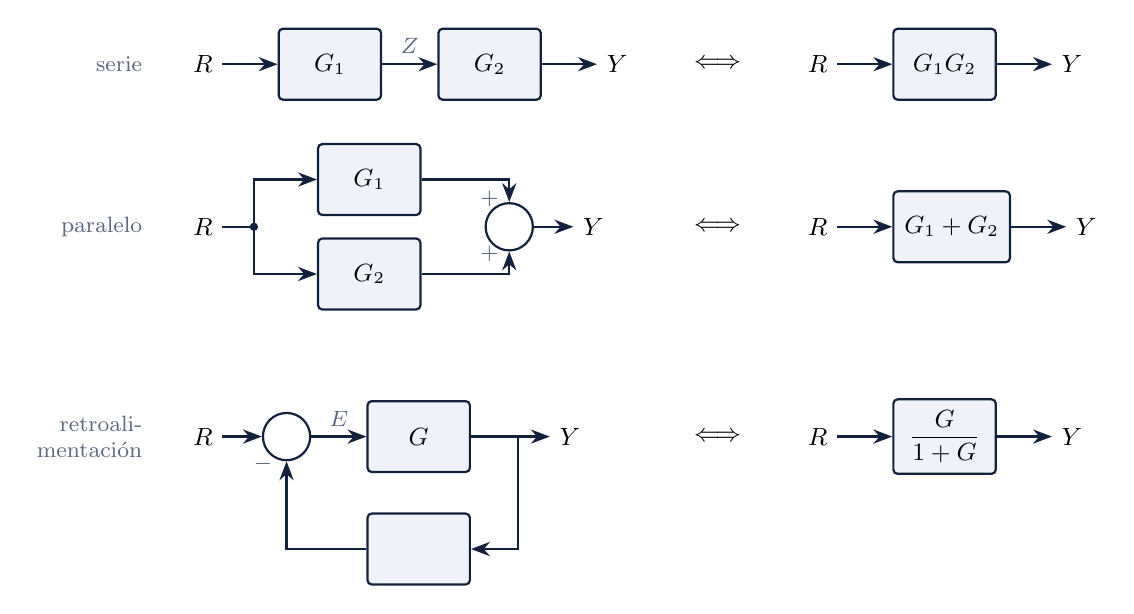
\begin{tikzpicture}[node distance=7mm]
  % serie
  \node (r1) {$R$}; \node[bloque,right=of r1] (a) {$G_1$}; \node[bloque,right=of a] (b) {$G_2$}; \node[right=of b] (y1) {$Y$};
  \draw[senal] (r1)--(a); \draw[senal] (a)--node[above,rot]{$Z$}(b); \draw[senal] (b)--(y1);
  \node[right=6mm of y1] (eq1) {$\Longleftrightarrow$};
  \node[right=6mm of eq1] (r1b) {$R$}; \node[bloque,right=of r1b] (ab) {$G_1G_2$}; \node[right=of ab] (y1b) {$Y$};
  \draw[senal] (r1b)--(ab); \draw[senal] (ab)--(y1b);
  \node[rot,left=4mm of r1] {serie};
  % paralelo
  \node[below=16mm of r1] (r2) {$R$}; \coordinate[right=4mm of r2] (n2); \fill[ctrlnoche] (n2) circle (1.5pt);
  \node[bloque,right=8mm of n2,yshift=6mm] (c) {$G_1$}; \node[bloque,right=8mm of n2,yshift=-6mm] (d) {$G_2$};
  \node[suma,right=8mm of c,yshift=-6mm] (S) {}; \node[right=5mm of S] (y2) {$Y$};
  \draw[thick,draw=ctrlnoche] (r2)--(n2); \draw[senal] (n2)|-(c); \draw[senal] (n2)|-(d); \draw[senal] (c)-|(S); \draw[senal] (d)-|(S); \draw[senal] (S)--(y2);
  \node[rot] at ($(S)+(-2.5mm,3.5mm)$) {$+$}; \node[rot] at ($(S)+(-2.5mm,-3.5mm)$) {$+$};
  \node at (eq1|-y2) (eq2) {$\Longleftrightarrow$};
  \node[right=6mm of eq2] (r2b) {$R$}; \node[bloque,right=of r2b] (cd) {$G_1+G_2$}; \node[right=of cd] (y2b) {$Y$};
  \draw[senal] (r2b)--(cd); \draw[senal] (cd)--(y2b);
  \node[rot,left=4mm of r2] {paralelo};
  % retroalimentación
  \node[below=22mm of r2] (r3) {$R$}; \node[suma,right=5mm of r3] (S3) {}; \node[bloque,right=of S3] (G) {$G$};
  \coordinate[right=6mm of G] (o3); \node[right=4mm of o3] (y3) {$Y$};
  \node[bloque,below=5mm of G] (H) {$\Hs$};
  \draw[senal] (r3)--(S3); \draw[senal] (S3)--node[above,rot]{$E$}(G); \draw[thick,draw=ctrlnoche] (G)--(o3); \draw[senal] (o3)--(y3);
  \draw[senal] (o3)|-(H); \draw[senal] (H)-|(S3); \node[rot] at ($(S3)+(-3mm,-3.5mm)$) {$-$};
  \node at (eq1|-y3) (eq3) {$\Longleftrightarrow$};
  \node[right=6mm of eq3] (r3b) {$R$}; \node[bloque,right=of r3b] (T) {$\dfrac{G}{1+G\Hs}$}; \node[right=of T] (y3b) {$Y$};
  \draw[senal] (r3b)--(T); \draw[senal] (T)--(y3b);
  \node[rot,left=4mm of r3,align=right] {retroali-\\mentación};
\end{tikzpicture}
\end{document}
